\documentclass[11pt]{article}

\usepackage[margin=1in]{geometry}
\usepackage{graphicx}
\usepackage{float}
\usepackage{amsmath,amssymb}
\usepackage{booktabs}
\usepackage{xcolor}
\usepackage[hidelinks]{hyperref}
\usepackage{caption}
\captionsetup{font=small}
\setlength{\parskip}{0.35em}

\graphicspath{{figures/}}

\title{\vspace{-1.5em}Transducer belief decomposition: what a transformer keeps and erases}
\author{Pritish Saha}
\date{\today}

\begin{document}
\maketitle
\vspace{-1.5em}

\noindent
This is a short report of what I have run so far on the transducer-decomposition direction from
\texttt{aim.md} \S10.4 and the coarse-graining picture from your worksheet. The question is whether
a transformer trained on a transducer's joint input/output stream builds the belief state in its
residual stream, and whether that belief separates into an input part and a transducer part.

\textbf{Headline result.} It does build the belief ($R^2\approx0.99$ on two processes), and whether
it \emph{separates} depends entirely on whether the intermediate token is observed. Observed, the
input and transducer beliefs are both cleanly readable. Hidden, they entangle, and
\textbf{coarse-graining the intermediate token erases 95--98\% of the input belief while the
transducer belief stays intact ($R^2\approx0.9$)} --- and this vanishes on a control where the
process is unpredictable. I show it on SNS and Fractal2. Every run is on a free Colab T4, so numbers
are at 100k training steps, not the full 1M.

\begin{center}
\fbox{\begin{minipage}{0.93\textwidth}
\textbf{Key results}
\begin{itemize}\itemsep1pt \setlength{\topsep}{2pt}
  \item Belief geometry is \textbf{linearly present} in the residual stream for transducers --- the
        full joint belief and both marginals, $R^2\approx0.99$, on two processes (SNS and Fractal2).
  \item Observing the intermediate token gives a \textbf{separable} (product) belief; hiding it gives
        an \textbf{entangled} one, exactly as the operator $\hat W=\sum_y\hat V$ predicts.
  \item Coarse-graining \textbf{erases 95--98\% of the input belief} while the transducer belief is
        \textbf{retained} ($R^2\approx0.9$); the effect \textbf{vanishes} when the process is
        unpredictable (control).
\end{itemize}
\end{minipage}}
\end{center}

\section{Setup}

An autonomous \textbf{input HMM} $\hat T^{(y)}$ (hidden states $R$) emits a symbol $y$; a
\textbf{transducer} $\hat U^{(x\mid y)}$ (hidden states $S$) reads $y$ and emits $x$. The observable
is the composite token $(y,x)$ and the joint state $(R,S)$ evolves under
$\hat V^{(y,x)} = \hat T^{(y)} \otimes \hat U^{(x\mid y)}$. Everything turns on \textbf{which tokens
the transformer sees}, one switch:
\begin{itemize}\itemsep1pt
  \item \texttt{joint}: train on $(y,x)$ (operator $\hat V$) --- beliefs are tensor products, so the
        input and transducer parts are \emph{separable}.
  \item \texttt{output\_only}: train on $x$ only (operator $\hat W^{(x)}=\sum_y\hat V^{(y,x)}$) ---
        the sum over the hidden $y$ \emph{entangles} $R$ and $S$, so the belief no longer factors.
  \item \texttt{input\_only}: train on $y$ only --- collapses to the input HMM's mixed states.
\end{itemize}
In all regimes the belief lives on the same $(R,S)$ space, so I always probe three targets: the
joint belief and its input and transducer marginals.

For each run I report five things. (1) The \textbf{entropy rate} of the observed process --- the
floor the cross-entropy loss can reach. (2) A \textbf{geometric probe}: least squares from the
residual stream to each belief, per layer and concatenated, as $R^2$/MSE, against an
untrained-network baseline. (3) A \textbf{predictive} check $d_\mu=\frac1L\sum_t
\mathrm{KL}(P_t\Vert Q_t)$ between the exact and the model's next-token distributions. (4) A
\textbf{separability fraction}: the share of analytical belief states that factor as a tensor
product ($1$ separable, $0$ fully entangled). (5) For the coarse-grained runs, an \textbf{erasure
cross-fit}: feed the $x$-only model the output stream and ask how well its residual stream recovers
the \emph{fully observable} belief --- low recovery is the information the transducer erased.

Model (Shai et al.\ App.\ A.6), shared across all runs: 4-layer causal transformer,
$d_{\text{model}}{=}64$, 1 head, $d_{\text{head}}{=}8$, $d_{\text{mlp}}{=}256$, context
$N_{\text{ctx}}{=}50$, ReLU, LayerNorm, $\sim$146k params, seed $42$. Next-token cross-entropy, SGD
(lr $0.01$, batch $64$), 100k steps. Analysis uses $10^4$ sampled sequences ($5\times10^5$
belief/activation pairs); controls are sequence-level CV, activation shuffle, and a
first-half/second-half temporal split.

The per-run process parameters are below. For the SNS the parameter is the self-loop probability
$p$; for Fractal2 it is the triple $(b,p,q)$; the transducer takes one parameter set per input
symbol. Hidden-state counts are $|R|$ (input) and $|S|$ (transducer); the observable vocabulary is
$4$ composite tokens under \texttt{joint} and $2$ output tokens under \texttt{output\_only}.

\begin{table}[H]\centering
\resizebox{\textwidth}{!}{%
\begin{tabular}{lllcc}
\toprule
run & input HMM & transducer (per input symbol) & $(|R|,|S|)$ & vocab (joint/out) \\
\midrule
IID $\to$ SNS          & IID, $p(y{=}1){=}0.5$        & SNS, $p\in\{0.35,\,0.80\}$ & $(1,2)$ & $4\,/\,2$ \\
SNS $\to$ SNS          & SNS, $p{=}0.5$               & SNS, $p\in\{0.35,\,0.80\}$ & $(2,2)$ & $4\,/\,2$ \\
Fractal2 $\to$ Fractal2 & Fractal2, $(0.85,0.5,0.5)$  & Fractal2, $(0.85,0.15,0.15),\,(0.85,0.85,0.85)$ & $(2,2)$ & $4\,/\,2$ \\
Fractal2 control       & Fractal2, $(0.5,0.5,0.5)$    & Fractal2, $(0.5,0.25,0.25),\,(0.5,0.75,0.75)$ & $(2,2)$ & $4$ \\
\bottomrule
\end{tabular}}
\caption{Per-run process configurations. All other hyperparameters are shared (above). The control
row is the degenerate Fractal2 ($b{=}0.5$) used in \S8.}
\end{table}

Each experiment below shows the same five plots, in order: the analytical belief manifolds; the
training curve; the per-layer probe; the controls; and the ground-truth-vs-readout comparison.

\section{Experiment 1 --- IID $\to$ SNS (validation, fully observable)}

The cleanest case: an IID input (single hidden state) carries no belief of its own, so the only
non-trivial target is the SNS transducer belief. The SNS is nonunifilar with a synchronizing
symbol, so its mixed states form a \emph{countable arc} on the 1-simplex --- an unambiguous target.

\begin{figure}[H]\centering
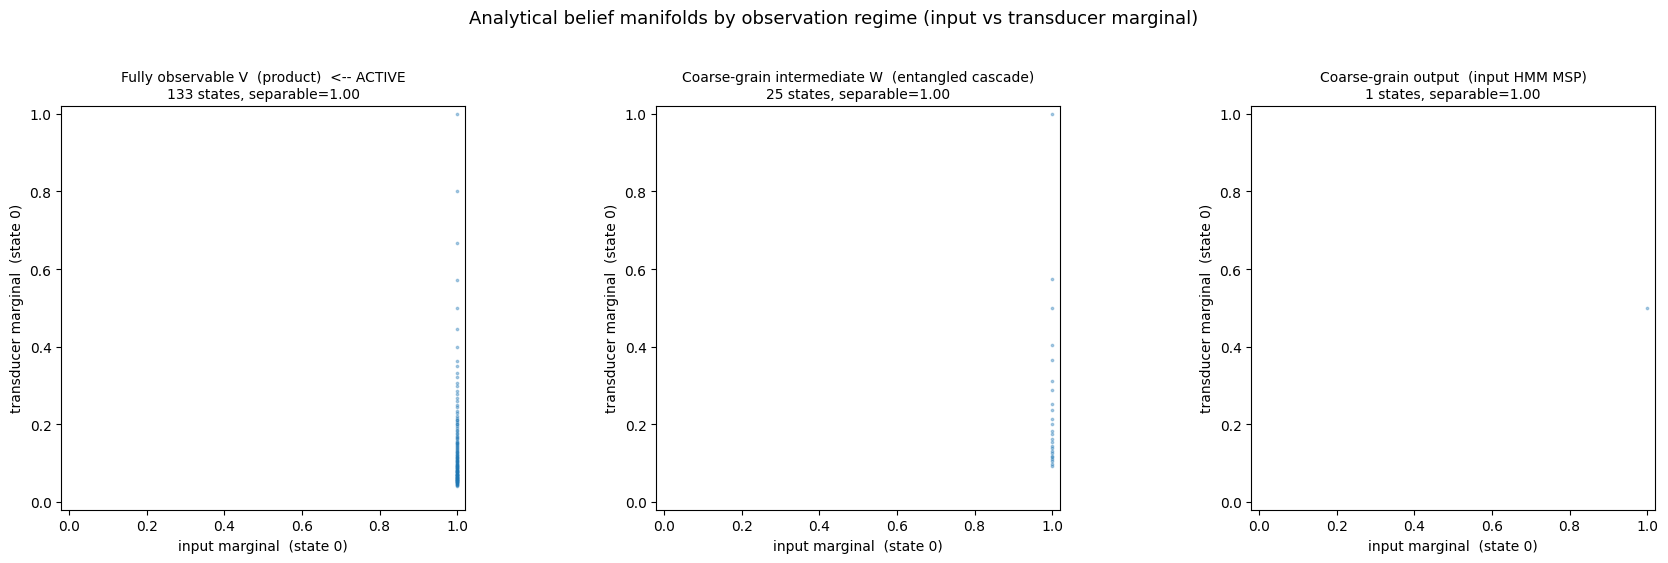
\includegraphics[width=\linewidth]{iid_sns_joint/fig_belief_manifolds.png}
\caption{\textbf{Analytical manifolds.} Input vs transducer marginal for the three regimes. With an
IID input the input marginal is constant, so everything sits on a vertical line; the transducer
coordinate traces the countable SNS arc. Nothing to entangle here (separability $1.0$ everywhere).}
\end{figure}

\begin{figure}[H]\centering
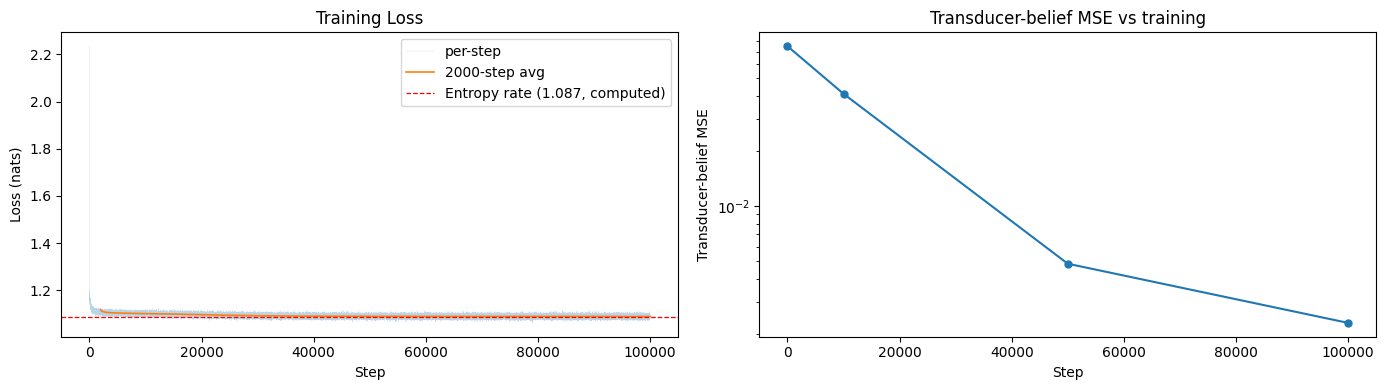
\includegraphics[width=\linewidth]{iid_sns_joint/fig_training.png}
\caption{\textbf{Training.} Loss converges to the entropy-rate floor $1.088$ (left; gap $+0.003$
nats, $d_\mu=0.0006$) --- the model predicts the process essentially optimally --- while the
transducer-belief MSE keeps dropping (right).}
\end{figure}

\begin{figure}[H]\centering
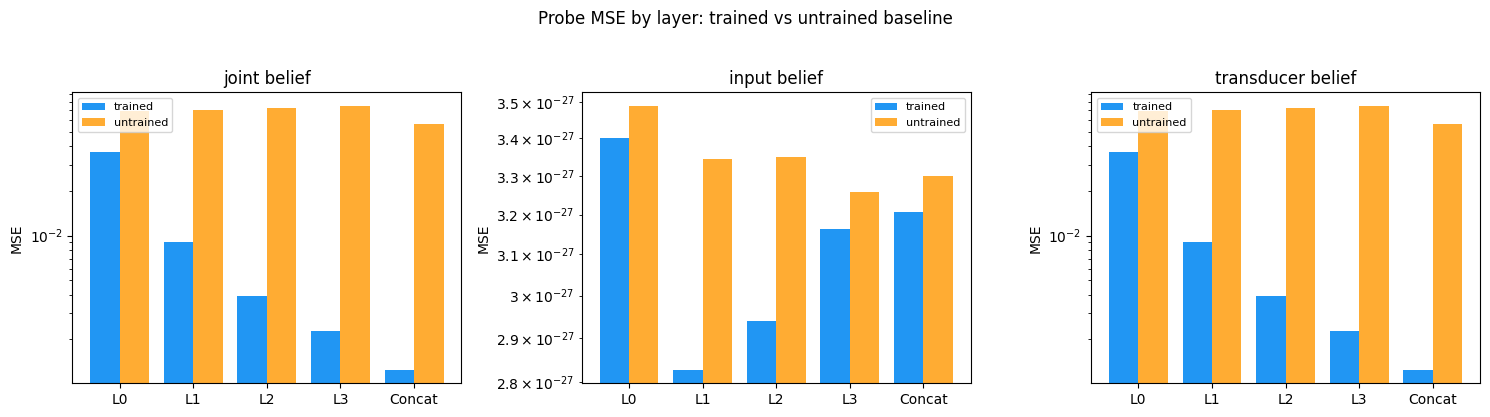
\includegraphics[width=\linewidth]{iid_sns_joint/fig_probes.png}
\caption{\textbf{Probe by layer.} Trained (blue) vs untrained (orange) MSE. The belief is refined
with depth and the concatenated probe reaches transducer $R^2=0.994$, far below the untrained
baseline ($R^2=0.73$).}
\end{figure}

\begin{figure}[H]\centering
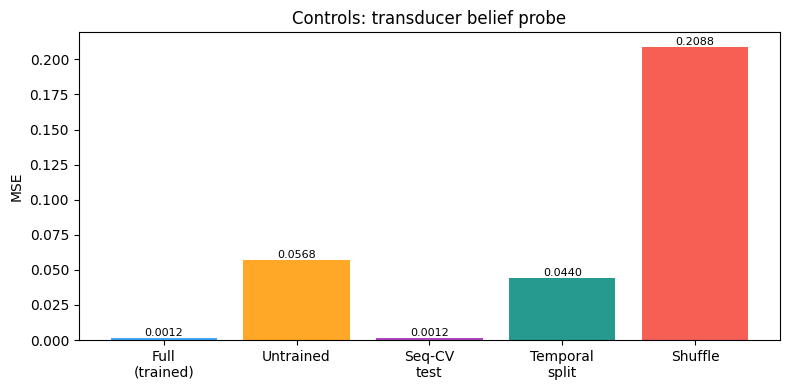
\includegraphics[width=\linewidth]{iid_sns_joint/fig_controls.png}
\caption{\textbf{Controls.} Shuffle degrades the fit $168\times$, the untrained net is $46\times$
worse, and sequence-level CV matches the full fit (no overfitting). The probe reads real structure.}
\end{figure}

\begin{figure}[H]\centering
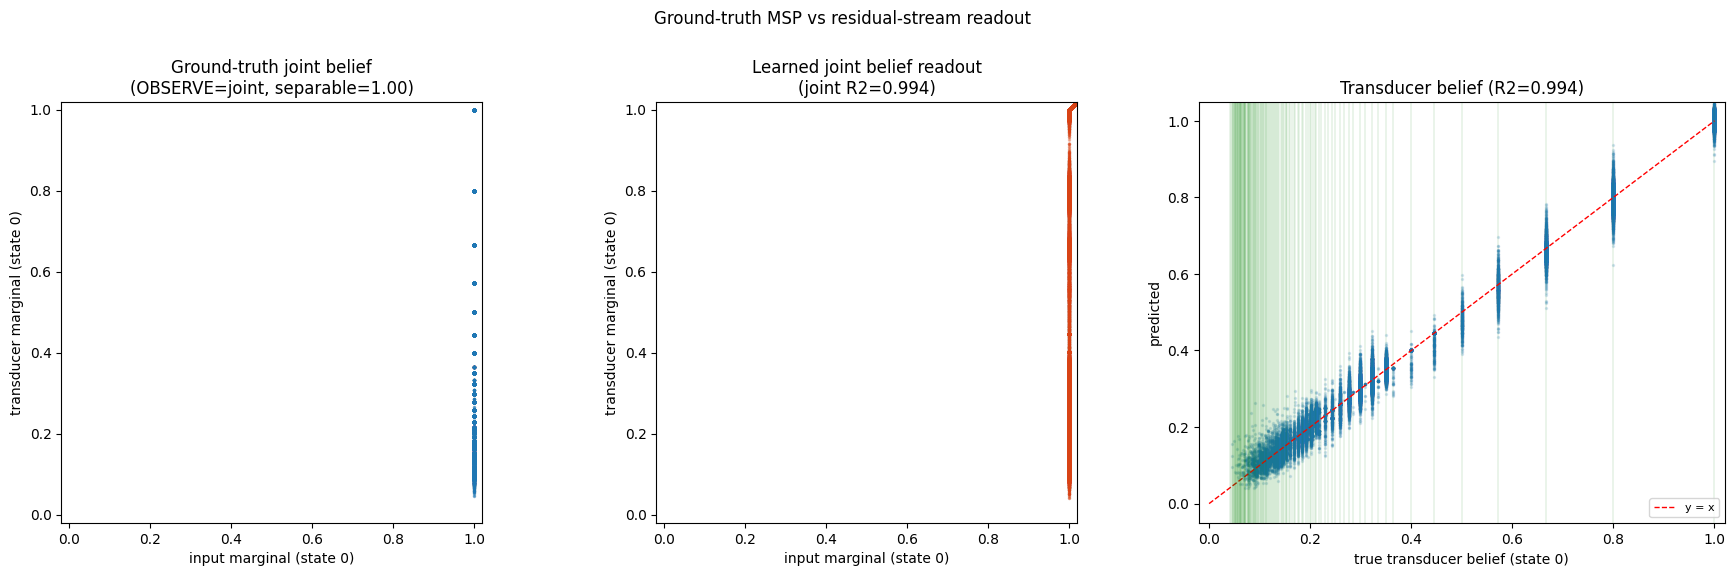
\includegraphics[width=\linewidth]{iid_sns_joint/fig_msp_vs_learned.png}
\caption{\textbf{Ground truth vs readout.} Right panel is decisive: predicted vs true transducer
belief on $y=x$ ($R^2=0.994$), landing on the countable SNS arc (green rug). The transformer has
reconstructed the exact belief manifold.}
\end{figure}

\noindent\textbf{Conclusion.} The pipeline works end to end: near-optimal prediction and a belief
manifold that is linearly present and lands on the right discrete set. This validates the machinery
before adding a structured input.

\section{Experiment 2 --- SNS $\to$ SNS, fully observable (\texttt{joint})}

Now the input is a 2-state SNS, so both an input belief and a transducer belief exist. Fully
observed, the joint belief is a clean product.

\begin{figure}[H]\centering

\includegraphics[width=\linewidth]{transducer_ckpt_sns_sns_joint/fig_belief_manifolds.png}
\caption{\textbf{Analytical manifolds (SNS$\to$SNS).} Left, fully observable $\hat V$: a 2-D
\emph{product} manifold (separability $1.00$). Middle, coarse-grained $\hat W$: a lower-dimensional
\emph{entangled} cascade (separability $0.34$). Right: the input HMM's mixed states. The active
regime here is the product (left).}
\end{figure}

\begin{figure}[H]\centering

\includegraphics[width=\linewidth]{transducer_ckpt_sns_sns_joint/fig_training.png}
\caption{\textbf{Training.} Loss $0.904$ at the floor $0.902$ (gap $+0.003$, $d_\mu=0.0011$). The
process is predictable (floor well below $\log 4=1.386$), so tracking beliefs helps prediction.}
\end{figure}

\begin{figure}[H]\centering

\includegraphics[width=\linewidth]{transducer_ckpt_sns_sns_joint/fig_probes.png}
\caption{\textbf{Probe by layer.} Both marginals are recovered cleanly when the intermediate token
is observed: concat $R^2 = 0.985$ (joint), $0.990$ (input), $0.992$ (transducer).}
\end{figure}

\begin{figure}[H]\centering

\includegraphics[width=\linewidth]{transducer_ckpt_sns_sns_joint/fig_controls.png}
\caption{\textbf{Controls.} Shuffle $127\times$, untrained $21\times$, seq-CV $\approx 1\times$. The
temporal split ($0.058$, $\sim$30$\times$) shows the linear map is somewhat position-specific
(absolute positional embeddings), as expected.}
\end{figure}

\begin{figure}[H]\centering

\includegraphics[width=\linewidth]{transducer_ckpt_sns_sns_joint/fig_msp_vs_learned.png}
\caption{\textbf{Ground truth vs readout.} The residual-stream readout (middle) reproduces the
product manifold; the transducer belief lies on $y=x$ ($R^2=0.992$).}
\end{figure}

\noindent\textbf{Conclusion.} With both tokens observed, the transformer holds the full joint belief
and \emph{both} marginals are separately readable ($R^2\approx0.99$). This is the separable baseline
against which the coarse-grained run is compared.

\section{Experiment 3 --- SNS $\to$ SNS, coarse-grained (\texttt{output\_only})}

Same process, but the model sees only $x$; the intermediate $y$ is hidden. It still tracks a belief
well --- but the \emph{entangled} one, and the erasure cross-fit shows what is lost.

\begin{figure}[H]\centering

\includegraphics[width=\linewidth]{transducer_ckpt_sns_sns_output_only/fig_belief_manifolds.png}
\caption{\textbf{Analytical manifolds}, same process; now the \emph{coarse-grained} $\hat W$ regime
(middle, separability $0.34$) is active --- the entangled cascade, not the product square.}
\end{figure}

\begin{figure}[H]\centering

\includegraphics[width=\linewidth]{transducer_ckpt_sns_sns_output_only/fig_training.png}
\caption{\textbf{Training.} Loss $0.469$ at the floor $0.470$ (gap $+0.001$, $d_\mu=0.0005$). The
$x$-only process is more predictable (fewer symbols, lower floor), and the model reaches it.}
\end{figure}

\begin{figure}[H]\centering

\includegraphics[width=\linewidth]{transducer_ckpt_sns_sns_output_only/fig_probes.png}
\caption{\textbf{Probe by layer.} The model's own (entangled) belief is recovered well: transducer
$R^2=0.995$, joint $0.992$. The input marginal ($0.978$) is a different, less informative quantity
than the fully observable input belief --- the point the cross-fit makes precise.}
\end{figure}

\begin{figure}[H]\centering

\includegraphics[width=\linewidth]{transducer_ckpt_sns_sns_output_only/fig_controls.png}
\caption{\textbf{Controls.} Robust under coarse-graining: shuffle $192\times$, untrained $19\times$,
seq-CV $\approx 1\times$.}
\end{figure}

\begin{figure}[H]\centering

\includegraphics[width=\linewidth]{transducer_ckpt_sns_sns_output_only/fig_msp_vs_learned.png}
\caption{\textbf{Ground truth vs readout.} The residual stream now reconstructs the entangled
cascade (middle), exactly the geometry $\hat W=\sum_y\hat V$ predicts when the intermediate token is
hidden.}
\end{figure}

\noindent\textbf{Erasure cross-fit.} From the $x$-only model, the fully observable \emph{transducer}
belief is recovered at $R^2=0.89$ (retained), but the fully observable \emph{input} belief at only
$R^2=0.05$ --- about \textbf{95\% erased}.
\textbf{Conclusion.} Hiding the intermediate token makes the driving process almost unreadable while
the transducer's own state stays legible in the output.

\section{Experiment 4 --- Fractal2 $\to$ Fractal2, fully observable (\texttt{joint})}

To check this is not specific to the SNS, I repeat with a Fractal2 source and transducer. (Fractal2
at $b{=}0.5$ is degenerate; I use $b{=}0.85$, which gives a predictable process --- entropy $0.92$,
well below $\log 4$; see the control.)

\begin{figure}[H]\centering

\includegraphics[width=\linewidth]{transducer_ckpt_fractal2_fractal2_joint/fig_belief_manifolds.png}
\caption{\textbf{Analytical manifolds (Fractal2$\to$Fractal2).} Fully observable (left) is a rich
product fractal (separability $1.00$); coarse-grained (middle) is a \emph{fully} entangled cascade
(separability $0.06$, far lower than the SNS's $0.34$).}
\end{figure}

\begin{figure}[H]\centering

\includegraphics[width=\linewidth]{transducer_ckpt_fractal2_fractal2_joint/fig_training.png}
\caption{\textbf{Training.} Loss $0.928$ at the floor $0.924$ (gap $+0.010$, $d_\mu=0.0015$).}
\end{figure}

\begin{figure}[H]\centering

\includegraphics[width=\linewidth]{transducer_ckpt_fractal2_fractal2_joint/fig_probes.png}
\caption{\textbf{Probe by layer.} Fully observable: input $R^2=0.997$, transducer $0.995$, joint
$0.994$ --- the belief geometry is cleanly linear on this process too.}
\end{figure}

\begin{figure}[H]\centering

\includegraphics[width=\linewidth]{transducer_ckpt_fractal2_fractal2_joint/fig_controls.png}
\caption{\textbf{Controls.} Shuffle $218\times$, untrained $32\times$, seq-CV $\approx 1\times$.
Notably the temporal split is tiny here ($0.007$, $\sim$3.5$\times$): Fractal2's belief direction is
far more position-invariant than the SNS's --- the same linear map works across context positions.}
\end{figure}

\begin{figure}[H]\centering

\includegraphics[width=\linewidth]{transducer_ckpt_fractal2_fractal2_joint/fig_msp_vs_learned.png}
\caption{\textbf{Ground truth vs readout.} The readout reproduces the product fractal (joint
$R^2=0.994$; transducer $R^2=0.995$ on $y=x$).}
\end{figure}

\noindent\textbf{Conclusion.} A second, structurally different process gives the same fully
observable result: the full joint belief and both marginals are linearly present at $R^2\approx0.99$.

\section{Experiment 5 --- Fractal2 $\to$ Fractal2, coarse-grained (\texttt{output\_only})}

The strongest erasure case: separability drops to $0.06$ (almost fully entangled).

\begin{figure}[H]\centering

\includegraphics[width=\linewidth]{transducer_ckpt_fractal2_fractal2_output_only/fig_belief_manifolds.png}
\caption{\textbf{Analytical manifolds}, same process; the coarse-grained $\hat W$ regime (middle,
separability $0.06$) is active --- a near-fully-entangled cascade.}
\end{figure}

\begin{figure}[H]\centering

\includegraphics[width=\linewidth]{transducer_ckpt_fractal2_fractal2_output_only/fig_training.png}
\caption{\textbf{Training.} Loss $0.473$ at the floor $0.471$ (gap $+0.004$, $d_\mu=0.0007$).}
\end{figure}

\begin{figure}[H]\centering

\includegraphics[width=\linewidth]{transducer_ckpt_fractal2_fractal2_output_only/fig_probes.png}
\caption{\textbf{Probe by layer.} Transducer belief recovered almost perfectly ($R^2=0.997$). The
input marginal has collapsed to a low-variance quantity ($R^2=0.28$ but tiny MSE): the $x$-only
observer of Fractal2 has almost no information about the driver even in its own belief.}
\end{figure}

\begin{figure}[H]\centering

\includegraphics[width=\linewidth]{transducer_ckpt_fractal2_fractal2_output_only/fig_controls.png}
\caption{\textbf{Controls.} Shuffle $294\times$ (the strongest of all runs), untrained $21\times$,
seq-CV $\approx 1\times$.}
\end{figure}

\begin{figure}[H]\centering

\includegraphics[width=\linewidth]{transducer_ckpt_fractal2_fractal2_output_only/fig_msp_vs_learned.png}
\caption{\textbf{Ground truth vs readout.} Residual-stream reconstruction of the entangled Fractal2
cascade (middle) and the transducer belief on $y=x$ ($R^2=0.997$, right).}
\end{figure}

\noindent\textbf{Erasure cross-fit.} The $x$-only model recovers the fully observable transducer
belief at $R^2=0.92$ (retained) but the fully observable input belief at only $R^2=0.017$ ---
about \textbf{98\% erased}, even more than the SNS, as the stronger entanglement predicts.
\textbf{Conclusion.} The effect replicates and intensifies: lower separability $\Rightarrow$ more
input erasure, transducer belief still kept.

\section{Control --- Fractal2 ($b{=}0.5$): the effect needs a predictable process}

As a sanity check I ran Fractal2$\to$Fractal2 at $b{=}0.5$. There the joint stream is maximally
random --- entropy rate exactly $\log 4$, the vocabulary bound --- so next-token prediction is
trivial and the model has no reason to build any belief. The probe collapses to the untrained
baseline (transducer $R^2=0.76$ vs untrained $0.73$; shuffle only $4\times$ instead of
$130$--$290\times$). So the whole phenomenon is contingent on the process being predictable; when it
is not, no belief geometry appears. (The notebook now flags any process whose entropy rate is near
$\log(\text{vocab})$, so this is caught before training.)

\section{Summary}

\begin{table}[H]\centering\small
\begin{tabular}{llccccc}
\toprule
process & regime & separ. & floor & CE$-h_\mu$ & probe $R^2$ (in / tr) & shuffle \\
\midrule
IID$\to$SNS          & joint        & 1.00 & 1.088 & $+0.003$ & --\ / 0.994 & $168\times$ \\
SNS$\to$SNS          & joint        & 1.00 & 0.902 & $+0.003$ & 0.990 / 0.992 & $127\times$ \\
SNS$\to$SNS          & output\_only & 0.34 & 0.470 & $+0.001$ & 0.978 / 0.995 & $192\times$ \\
Fractal2$\to$Fr.\    & joint        & 1.00 & 0.924 & $+0.010$ & 0.997 / 0.995 & $218\times$ \\
Fractal2$\to$Fr.\    & output\_only & 0.06 & 0.471 & $+0.004$ & 0.280 / 0.997 & $294\times$ \\
Fractal2 ($b{=}0.5$) & joint        & 1.00 & $\log 4$ & $\approx 0$ & --\ / 0.76 & $4\times$ \\
\bottomrule
\end{tabular}
\caption{Belief recovery and prediction. ``probe $R^2$'' is the concatenated-layer fit to the input
and transducer marginals (in the coarse-grained rows these are the model's own entangled belief).}
\end{table}

\begin{table}[H]\centering\small
\begin{tabular}{lccc}
\toprule
coarse-grained process & separability & full \textbf{input} $R^2$ & full \textbf{transducer} $R^2$ \\
\midrule
SNS$\to$SNS           & 0.34 & 0.05\phantom{0} \; ($\sim$95\% erased) & 0.89 \; (retained) \\
Fractal2$\to$Fractal2 & 0.06 & 0.017 \; ($\sim$98\% erased)          & 0.92 \; (retained) \\
\bottomrule
\end{tabular}
\caption{Erasure cross-fit: how much of the \emph{fully observable} belief the $x$-only model
recovers. The input belief is almost entirely erased; the transducer belief is kept.}
\end{table}

\section{What this says}

Three things come out cleanly. First, the belief-state-in-residual-stream result extends from plain
HMMs to transducers: with the joint input/output stream observed, the transformer linearly encodes
the full joint belief and both marginals separate cleanly ($R^2\approx0.99$ on two different
processes). Second, hiding the intermediate token entangles the two latent spaces exactly as the
modified operator $\hat W=\sum_y\hat V$ predicts, and the transformer follows that entangled geometry
rather than the product one. Third, and most concretely, coarse-graining \textbf{erases the input
belief} (95--98\% across the two processes) while \textbf{keeping the transducer belief} --- so
``how much does the transducer erase'' has a clear quantitative answer, and more entanglement means
more erasure. The control shows this is a real, contingent effect: it only appears when the process
is predictable enough that tracking beliefs helps prediction.

Natural next steps are a third process (Mess3 driving an SNS) to confirm the pattern once more, the
full 1M-step runs for tighter numbers, and the feedback / partially observable setting, where each
agent carries the modified-operator mixed states from your worksheet.

\end{document}
